\documentclass[11pt,letterpaper]{article}
\usepackage[
    lmargin=2.2in,
    rmargin=0.7in,
    tmargin=1.0in,
    bmargin=1.0in
]{geometry}
\usepackage{notes}
\usetikzlibrary{decorations.markings}

\begin{document}

\begin{center}
\Large\textbf{DAY 29 -- Vector Functions and Linear Systems}\\
\normalsize (Section 4.2)
\end{center}

%%%%%%%%%%%%%%%%%%%%%%%%%%%%%%%%%%%%%%%%%%%%%%%%%%%%%%%%%%%%%%%%%%%%%%%%
\section{Systems of Differential Equations}

\subsection{Goal of Chapter 4}
In the last lecture, we learned how to solve linear systems of the form
$$
\begin{pmatrix}
    a & b\\
    c & d
\end{pmatrix} \begin{pmatrix}
    x\\y 
\end{pmatrix} = \begin{pmatrix}
    f\\g
\end{pmatrix},
$$
where the solution $x$ and $y$ are numbers. The main goal in Chapter 4 is to learn how to solve \textbf{linear systems of differential equations} with constant coefficients:
\begin{equation}    
\begin{dcases}
x'=ax+by,\\
y'=cx+dy
\end{dcases},\label{1}
\end{equation}
where the unknowns $x(t)$ and $y(t)$ are \textit{functions}. Then we will learn how to visualize these solutions.

\subsection{Matrix Form}
We combine these functions into one \textbf{vector-valued function}
\[
\mathbf{x}(t)=
\begin{pmatrix}x(t)\\y(t)\end{pmatrix}.
\]
Using matrix-vector multiplication, the system \eqref{1} can be rewritten as 
\[
\begin{pmatrix}x'\\y'\end{pmatrix}
=
\begin{pmatrix}
a&b\\c&d
\end{pmatrix}
\begin{pmatrix}x\\y\end{pmatrix}, \qquad \text{or} \qquad \mathbf{x}'=A\mathbf{x}.
\]
There are several advantages to writing the system in matrix form. Most of the advantages will be explained later. For now, let us practice putting an equation in this form.

\begin{example}[1]{
Rewrite the system in matrix form:
\[
\begin{dcases}
x'=-3x+2y,\\
y'=-4x+3y.
\end{dcases}
\]
}

\paragraph{Step 1. Define the vector function.}
Let
\[
\mathbf{x}(t)=
\begin{pmatrix}x(t)\\y(t)\end{pmatrix},
\quad \text{then its derivative is}\quad 
\mathbf{x}'(t)=
\begin{pmatrix}x'(t)\\y'(t)\end{pmatrix}.
\]

\paragraph{Step 2. Collect the coefficients.}
The first equation gives the first row of $A$;
the second equation gives the second row. Thus, by matrix-vector multiplication
\[
\boxed{
\mathbf{x}'=
\begin{pmatrix}
-3&2\\-4&3
\end{pmatrix}\mathbf{x}.
}
\]
\end{example}

% TRANSITION 1:
% Explain that before finding solutions, we need to know
% how to differentiate a vector function and check a formula.

%-------------------------------------------------------------
\subsection{Verifying a Solution}

Before learning how to solve a system, we will practice
checking a proposed solution. One of the advantages of the matrix form is that the given solution is easy to verify. To verify the solution to $\mathbf{x}'=A\mathbf{x}$
\begin{enumerate}
    \item Compute the LHS: differentiate to compute $\mathbf{x}'(t)$.
    \item Compute the RHS: multiply to compute $A\mathbf{x}(t)$.
    \item Compare: check that the two vectors agree for all $t$.
\end{enumerate}

\begin{example}[2]{
Show that
\[
\mathbf{x}(t)=e^{-t}
\begin{pmatrix}1\\1\end{pmatrix}
\]
is a solution to the system
\[
\mathbf{x}'=
\begin{pmatrix}
-3&2\\-4&3
\end{pmatrix}\mathbf{x}.
\]
}
\paragraph{Step 1. Compute the LHS.} Since the derivative of $e^{-t}$ is $-e^{-t}$, we have
\[
\mathbf{x}'(t)
=-e^{-t}\begin{pmatrix}1\\1\end{pmatrix}
=e^{-t}\begin{pmatrix}-1\\-1\end{pmatrix}.
\]

\paragraph{Step 2. Compute the RHS.} Take the function $e^{-t}$ off to the side. Then carry out the usual matrix-vector multiplication
\[
A\mathbf{x}(t)
=e^{-t}
\begin{pmatrix}
-3&2\\-4&3
\end{pmatrix}
\begin{pmatrix}1\\1\end{pmatrix}
=e^{-t}
\begin{pmatrix}
-3+2\\-4+3
\end{pmatrix}
=e^{-t}
\begin{pmatrix}-1\\-1\end{pmatrix}.
\]

\paragraph{Step 3. Compare.}
The two expressions agree:
\[
\boxed{\mathbf{x}'(t)=A\mathbf{x}(t).}
\]
Therefore, the proposed vector function is a solution.
\end{example}

%-------------------------------------------------------------
The solution is the vector function 
$$
    \textbf{x}(t) = \begin{pmatrix}
        e^{-t}\\
        e^{-t}
    \end{pmatrix}.
$$
This function traces out a path in the 2D plane. What does this path look like?


% ADD:
% Evaluate the solution from Example 2 at t=0.
% This connects the abstract initial condition to (1,1).

% TRANSITION 2:
% We have checked the solution algebraically.
% Now ask what the solution looks like as time changes.

%%%%%%%%%%%%%%%%%%%%%%%%%%%%%%%%%%%%%%%%%%%%%%%%%%%%%%%%%%%%%%%%%%%%%%%%
\section{Visualizing Vector Solutions}

\subsection{Definitions}

It is helpful to think of the function 
\[
\mathbf{x}(t)=
\begin{pmatrix}
x(t)\\y(t)
\end{pmatrix}.
\]
as a point $(x(t),y(t))$ in the plane that moves with time $t$. Therefore $\textbf{x}(t)$ traces out a path in the $xy$-plane. The path has many names: \textbf{plane curve}, \textbf{trajectory}, or \textbf{orbit}. In Calculus III, you may have used the notation $\mathbf{r}(t)=\langle x(t),y(t)\rangle$. This is the same concept with different notation.

The plane curve may connect two points $\textbf{a}$ and $\textbf{b}$. We want to distinguish whether the point $(x(t),y(t))$ is moving from $\textbf{a}$ to $\textbf{b}$, or from $\textbf{b}$ to $\textbf{a}$.  The direction as time increases is indicated by placing arrows on the curves. This is called the \textbf{orientation} of the curve. The $xy$-plane on which the orbit is plotted in is called the \textbf{phase plane}.

\begin{center}
\begin{tikzpicture}[
    x=1cm,y=1cm,
    >=Stealth,
    every node/.style={font=\small}
]
    % Axes
    \draw[->] (-2.4,0) -- (3.5,0) node[right] {$x$};
    \draw[->] (0,-0.5) -- (0,3.3) node[above] {$y$};

    % Endpoints and a point on the curve
    \coordinate (a) at (-1.9,1.1);
    \coordinate (p) at (2.1,1.2);
    \coordinate (b) at (2.8,2.7);

    % Curve, oriented from a toward b
    \draw[
        thick,
        postaction={decorate},
        decoration={
            markings,
            mark=at position 0.55 with {\arrow{Stealth}}
        }
    ]
        (a)
        .. controls (-1.4,2.6) and (-0.8,1.0) .. (0.8,1.0)
        .. controls (1.3,1.0) and (1.7,1.0) .. (p)
        .. controls (2.6,1.45) and (2.9,2.0) .. (b);

    % Endpoints
    \node at (-1.8,3) {phase plane};
    \fill (a) circle (2pt);
    \fill (b) circle (2pt);
    \node[left] at (a) {$\mathbf{a}$};
    \node[above right] at (b) {$\mathbf{b}$};

    % Orientation label
    \node[below] at (0.9,0.85) {orientation};

    % Tangent vector at p
    % Direction matches the curve's tangent: (1,0.5)
    \fill (p) circle (2pt);
    \draw[->,blue,very thick]
        (p) -- (3.3,1.8)
        node[ right] {$\mathbf{x}'(t)$};

    \node[below right] at (p) {$\mathbf{x}(t)$};
    \node[blue,above] at (2.8,2.05) {tangent vector};
\end{tikzpicture}
\end{center}



\subsection{Analysis Tools}

To sketch a vector function
\[
\mathbf{x}(t)=
\begin{pmatrix}x(t)\\y(t)\end{pmatrix}, \quad t\in(a,b)
\]
we want to determine the curve's shape and its orientation.
We will use four tools from Calculus III.

\paragraph{1. Plotting points.} 
For any value of $t_0\in(a,b)$, evaluating $\textbf{x}(t_0)=(x(t_0),y(t_0))$ gives one coordinate in the path of $\textbf{x}(t)$. It can be helpful to choose a few values of $t$ and plot its representative coordinate. For example, you can substitute $t=0$ to quickly obtain a reference point $(x_0,y_0)$. 

\paragraph{2. Parameter elimination.}
When possible, combine the two functions $x=x(t)$ and $y=y(t)$
to obtain an equation involving only $x$ and $y$. The goal is to eliminate the $t$ variable.
For example, suppose $x(t)=t$ and $y(t)=t^2$. Then 
\[
y=t^2=x^2.
\]
This reveals the curve's shape: the plane curve lies along the parabola $y=x^2$.

\paragraph{3. Tangent vector.}
Differentiate each component to find the
\textbf{velocity} or \textbf{tangent vector}:
\[
\mathbf{x}'(t)=
\begin{pmatrix}x'(t)\\y'(t)\end{pmatrix}.
\]
When $\mathbf{x}'(t)\ne\mathbf{0}$, this vector is
tangent to the curve and points in the direction of motion.
The signs of its components tell us how the particle moves:
\[
\begin{array}{l|l}
x'(t)>0:\ \text{right} & x'(t)<0:\ \text{left}\\
\hline
y'(t)>0:\ \text{up}    & y'(t)<0:\ \text{down}
\end{array}
\]
Evaluating $\mathbf{x}'(t)$ at a convenient time helps
us place an orientation arrow on the curve.

\paragraph{4. Limits.}
Take limits of each component to determine where the
particle goes as $t$ approaches an endpoint or infinity:
\[
\lim_{t\to\infty}\mathbf{x}(t)
=
\begin{pmatrix}
\displaystyle\lim_{t\to\infty}x(t)\\[2mm]
\displaystyle\lim_{t\to\infty}y(t)
\end{pmatrix},
\]
provided both component limits exist.
For example, if $x(t)\to0$ and $y(t)\to0$, the
particle approaches the origin. If a component grows
without bound, the particle moves off to infinity.

Together, these tools tell us \textit{the shape of the curve},
\textit{which direction it moves}, and \textit{where it ends up}.

\subsection{A Sketching Procedure}

To sketch a vector function $\textbf{v}(t)=((x(t),y(t))$:
\begin{enumerate}
    \item Identify the curve by relating $x$ and $y$.
    \item Find a few points, such as $\mathbf{x}(0)$.
    \item Indicate the orientation using increasing
    values of $t$ or a velocity vector.
    \item Check limits when needed to determine which
    portion of the curve is traced.
\end{enumerate}

Limits are also computed component-by-component:
\[
\lim_{t\to a}\mathbf{x}(t)=
\begin{pmatrix}
\displaystyle\lim_{t\to a}x(t)\\[2mm]
\displaystyle\lim_{t\to a}y(t)
\end{pmatrix},
\]
provided both component limits exist.

%%%%%%%%%%%%%%%%%%%%%%%%%%%%%%%%%%%%%%%%%%%%%%%%%%%%%%%%%%%%%%%%%%%%%%%%
\section{Sketching Plane Curves}


%-------------------------------------------------------------
\subsection{Lines}

The vector function
\[
\mathbf{x}(t)=t\mathbf{v}+\mathbf{b},
\qquad t\in\mathbb R,
\]
traces a straight line, where $\mathbf{v}\ne\mathbf{0}$
and $\mathbf{b}$ are constant vectors.
The vector $\mathbf{b}=\mathbf{x}(0)$ gives a point
on the line, while $\mathbf{v}=\mathbf{x}'(t)$ gives
its direction and orientation.

Because $t$ ranges over all real numbers, the particle
traces the entire line.

\begin{example}[3]{
Sketch the plane curve and indicate its orientation:
\[
\mathbf{x}(t)=
t\begin{pmatrix}2\\-4\end{pmatrix}
+\begin{pmatrix}2\\2\end{pmatrix},
\qquad t\in\mathbb R.
\]
}

\paragraph{Step 1. Points.}
Substituting $t=0$ and $t=1$ gives
\[
\mathbf{x}(0)=\begin{pmatrix}2\\2\end{pmatrix},
\qquad
\mathbf{x}(1)=\begin{pmatrix}4\\-2\end{pmatrix}.
\]
The line passes through $(2,2)$ and $(4,-2)$.
As time increases from $0$ to $1$, the particle
moves from the first point to the second.

\paragraph{Step 2. Shape.}
The components are
\[
x=2t+2,\qquad y=-4t+2.
\]
Solving the first equation for $t$ and substituting
into the second gives
\[
t=\frac{x-2}{2}
\quad\Longrightarrow\quad
y=-4\left(\frac{x-2}{2}\right)+2=-2x+6.
\]
Therefore, the curve lies on the line
\[
\boxed{y=-2x+6.}
\]

\paragraph{Step 3. Tangent.}
The tangent vector is constant:
\[
\mathbf{x}'(t)=\begin{pmatrix}2\\-4\end{pmatrix}.
\]
The particle moves $2$ units to the right and $4$ units
down for each unit increase in time. Thus, the
orientation is \textbf{downward and to the right}.

\paragraph{Step 4. Limits.}
The component limits are
\[
\begin{array}{c|cc}
 & x(t) & y(t)\\
\hline
t\to-\infty & -\infty & +\infty\\
t\to+\infty & +\infty & -\infty
\end{array}
\]
The particle does not approach a finite point in
either direction. Its path extends indefinitely
along the line.

\begin{center}
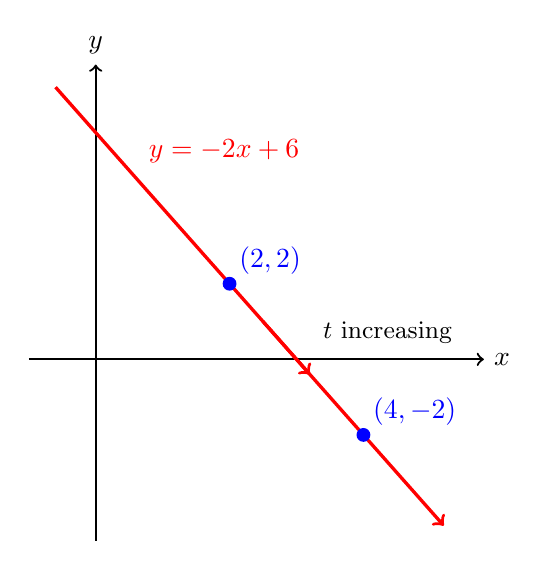
\begin{tikzpicture}[x=0.85cm,y=0.48cm]
    % Axes
    \draw[->,thick] (-1,0) -- (5.8,0)
        node[right] {$x$};
    \draw[->,thick] (0,-4.8) -- (0,7.8)
        node[above] {$y$};

    % Entire line: arrows at both ends indicate continuation
    \draw[->,red,very thick]
        (-0.6,7.2) -- (5.2,-4.4);

    % Interior arrow indicates increasing time
    \draw[->,red,very thick]
        (2.5,1) -- (3.2,-0.4);
    \node[right] at (3.25,0.7)
        {\small $t$ increasing};

    % Points at t=0 and t=1
    \fill[blue] (2,2) circle (2.5pt);
    \node[above right,blue] at (2,2)
        {$(2,2)$};

    \fill[blue] (4,-2) circle (2.5pt);
    \node[above right,blue] at (4,-2)
        {$(4,-2)$};

    % Line label
    \node[red,right] at (0.65,5.5)
        {$y=-2x+6$};
\end{tikzpicture}
\end{center}
\end{example}
%-------------------------------------------------------------
\subsection{Rays}

Replacing $t$ with an exponential changes which part
of a line is traced. Consider
\[
\mathbf{x}(t)=e^{\lambda t}\mathbf{v},
\qquad t\in\mathbb R,
\]
where $\mathbf{v}\ne\mathbf{0}$ and $\lambda\ne0$.

Since $e^{\lambda t}>0$, the position is always a
positive multiple of $\mathbf{v}$. As $t$ ranges over
$\mathbb R$, the exponential takes every positive value.
Thus, the curve traces a \textbf{ray} in the direction
of $\mathbf{v}$, excluding the origin.

The vector $\mathbf{v}$ determines the ray.
The sign of $\lambda$ determines its orientation:
\begin{itemize}
    \item $\lambda>0$: the particle moves
    \textbf{away from} the origin.
    \item $\lambda<0$: the particle moves
    \textbf{toward} the origin.
\end{itemize}
If $\lambda=0$, the function is constant:
$\mathbf{x}(t)=\mathbf{v}$. These straight trajectories are called
\textbf{linear orbits}. They will play an important
role when we solve $\mathbf{x}'=A\mathbf{x}$.

%-------------------------------------------------------------
\begin{example}[4]{
Sketch the plane curve and indicate its orientation:
\[
\mathbf{x}(t)=e^t
\begin{pmatrix}2\\4\end{pmatrix},
\qquad t\in\mathbb R.
\]
}

\paragraph{Step 1. Points.}
At $t=0$,
\[
\mathbf{x}(0)=
\begin{pmatrix}2\\4\end{pmatrix}.
\]
The particle passes through $(2,4)$.

\paragraph{Step 2. Shape.}
The components are
\[
x=2e^t,\qquad y=4e^t.
\]
We can determine the shape by dividing $y/x$:
$$
\frac{y}{x}=\frac{4e^t}{2e^t}=2\implies y=2x.
$$
Therefore, the ray lies somewhere along the line
\[
\boxed{y=2x.}
\]

\paragraph{Step 3. Tangent.}
Differentiating gives
\[
\mathbf{x}'(t)=e^t
\begin{pmatrix}2\\4\end{pmatrix}.
\]
Both components are positive, so the particle moves
\textbf{upward and to the right}, away from the origin.

\paragraph{Step 4. Limits.}
As $t\to-\infty$,
\[
\mathbf{x}(t)\to
\begin{pmatrix}0\\0\end{pmatrix}.
\]
As $t\to\infty$, both components increase without bound.
The origin is approached but never reached at a
finite time, so we mark it with an open circle.

\begin{center}
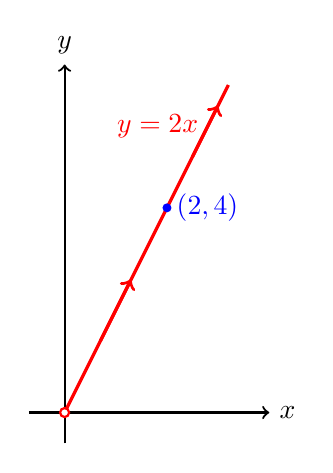
\begin{tikzpicture}[scale=0.65]
    % Axes
    \draw[->,thick] (-0.7,0) -- (4,0)
        node[right] {$x$};
    \draw[->,thick] (0,-0.6) -- (0,6.8)
        node[above] {$y$};

    % Ray
    \draw[red,very thick] (0,0) -- (3.2,6.4);

    % Orientation: increasing time
    \draw[->,red,very thick] (0.7,1.4) -- (1.3,2.6);
    \draw[->,red,very thick] (2.5,5) -- (3,6);

    % Excluded endpoint and reference point
    \draw[red,fill=white,thick] (0,0) circle (2.5pt);
    \fill[blue] (2,4) circle (2.5pt);
    \node[right,blue] at (2,4) {$(2,4)$};

    \node[left,red] at (2.8,5.6) {$y=2x$};
\end{tikzpicture}
\end{center}
\end{example}

%-------------------------------------------------------------
\paragraph{Shifting the ray.}
Adding a constant vector translates the path:
\[
\mathbf{x}(t)=e^{\lambda t}\mathbf{v}+\mathbf{b}.
\]
The ray now extends from $\mathbf{b}$ in the direction
of $\mathbf{v}$, excluding $\mathbf{b}$ itself.
For $\lambda>0$, the particle moves away from
$\mathbf{b}$; for $\lambda<0$, it moves toward
$\mathbf{b}$.

% Suggested lecture skip: leave Example 5 for students to read.
\begin{example}[5]{
Sketch the plane curve and indicate its orientation:
\[
\mathbf{x}(t)=e^{-2t}
\begin{pmatrix}-3\\1\end{pmatrix}
+\begin{pmatrix}1\\-1\end{pmatrix},
\qquad t\in\mathbb R.
\]
}

\paragraph{Step 1. Points.}
At $t=0$,
\[
\mathbf{x}(0)=
\begin{pmatrix}-3\\1\end{pmatrix}
+\begin{pmatrix}1\\-1\end{pmatrix}
=
\begin{pmatrix}-2\\0\end{pmatrix}.
\]
The particle passes through $(-2,0)$.

\paragraph{Step 2. Shape.}
The components are
\[
x=1-3e^{-2t},
\qquad
y=-1+e^{-2t}.
\]
We can divide $y+1$ by $x-1$: 
\[
\frac{y+1}{x-1}=\frac{e^{-2t}}{-3e^{-2t}}=-\frac{1}{3},
\]
which means the shape is
\[
\boxed{y+1=-\frac13(x-1)}
\]
This is a line with slope $m=-1/3$ through the point $(1,-1)$.

\paragraph{Step 3. Tangent.}
Differentiating gives
\[
\mathbf{x}'(t)
=-2e^{-2t}\begin{pmatrix}-3\\1\end{pmatrix}
=e^{-2t}\begin{pmatrix}6\\-2\end{pmatrix}.
\]
The particle moves \textbf{downward and to the right},
toward $(1,-1)$.

\paragraph{Step 4. Limits.}
As $t\to\infty$, the exponential decays to zero:
\[
\lim_{t\to\infty}\mathbf{x}(t)
=\begin{pmatrix}1\\-1\end{pmatrix}.
\]
As $t\to-\infty$, $x(t)\to-\infty$ and
$y(t)\to+\infty$.
The point $(1,-1)$ is approached but never reached
at a finite time.

\begin{center}
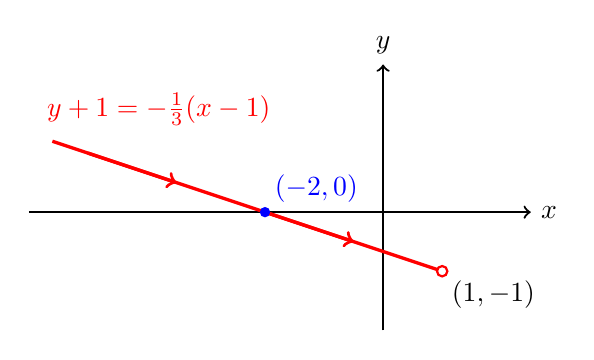
\begin{tikzpicture}[scale=0.75]
    % Axes
    \draw[->,thick] (-6,0) -- (2.5,0)
        node[right] {$x$};
    \draw[->,thick] (0,-2) -- (0,2.5)
        node[above] {$y$};

    % Shifted ray
    \draw[red,very thick] (-5.6,1.2) -- (1,-1);

    % Orientation: increasing time, toward the endpoint
    \draw[->,red,very thick] (-5,1) -- (-3.5,0.5);
    \draw[->,red,very thick] (-2,0) -- (-0.5,-0.5);

    % Reference point
    \fill[blue] (-2,0) circle (2.5pt);
    \node[above right,blue] at (-2,0) {$(-2,0)$};

    % Excluded endpoint
    \draw[red,fill=white,thick] (1,-1) circle (2.5pt);
    \node[below right] at (1,-1) {$(1,-1)$};

    \node[above,red] at (-3.8,1.3)
        {$y+1=-\frac13(x-1)$};
\end{tikzpicture}

\small
The ray extends in the direction $\mathbf{v}$,
but the particle moves toward $\mathbf{b}$.
\end{center}
\end{example}

%-------------------------------------------------------------
\subsection{Circles and Ellipses}

The vector function
\[
\mathbf{x}(t)=
\begin{pmatrix}
\rho\cos t\\
\rho\sin t
\end{pmatrix},
\qquad \rho>0,
\]
traces a circle. Using the identity
$\cos^2t+\sin^2t=1$, we obtain
\[
x^2+y^2
=\rho^2\cos^2t+\rho^2\sin^2t
=\rho^2.
\]
Thus, the curve is a circle centered at the origin
with radius $\rho$. More generally,
\[
\mathbf{x}(t)=
\begin{pmatrix}
\alpha\cos t\\
\beta\sin t
\end{pmatrix},
\qquad \alpha,\beta>0,
\]
traces an ellipse. The constants $\alpha$ and $\beta$
give its horizontal and vertical semiaxis lengths.

\begin{example}[6]{
Sketch the plane curve and indicate its orientation:
\[
\mathbf{x}(t)=
\begin{pmatrix}
4\cos t\\
2\sin t
\end{pmatrix},
\qquad t\ge0.
\]
}

\paragraph{Step 1. Points.}
Evaluating at quarter-period intervals gives
\[
\begin{array}{c|cccc}
t & 0 & \pi/2 & \pi & 3\pi/2\\
\hline
(x(t),y(t)) & (4,0) & (0,2) & (-4,0) & (0,-2)
\end{array}
\]
These are the four intercepts of the curve.

\paragraph{Step 2. Shape.}
Since $x=4\cos t$ and $y=2\sin t$, we eliminate
the parameter using the identity
$\cos^2t+\sin^2t=1$:
\[
\frac{x^2}{16}+\frac{y^2}{4}
=\cos^2t+\sin^2t=1.
\]
Thus, the curve is the ellipse
\[
\boxed{\frac{x^2}{16}+\frac{y^2}{4}=1.}
\]

\paragraph{Step 3. Tangent.}
Differentiating gives
\[
\mathbf{x}'(t)=
\begin{pmatrix}
-4\sin t\\
2\cos t
\end{pmatrix}.
\]
At the top of the ellipse,
\[
\mathbf{x}\left(\frac{\pi}{2}\right)
=\begin{pmatrix}0\\2\end{pmatrix},
\qquad
\mathbf{x}'\left(\frac{\pi}{2}\right)
=\begin{pmatrix}-4\\0\end{pmatrix}.
\]
The tangent vector points left, so the orientation
is \textbf{counterclockwise}.

\paragraph{Step 4. Limit.}
There is no limiting position as $t\to\infty$.
The particle continues around the ellipse,
repeating its motion every $2\pi$ units of time.

\begin{center}
% Requires \usetikzlibrary{decorations.markings}
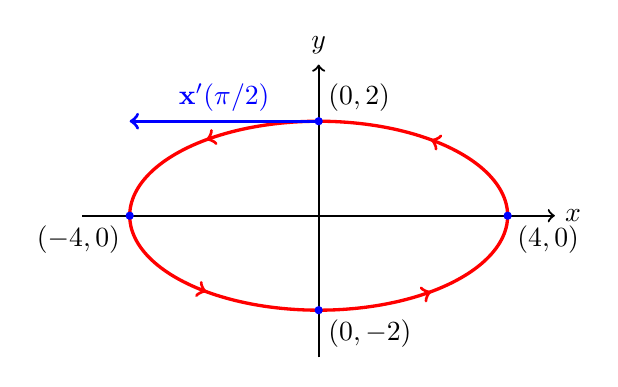
\begin{tikzpicture}[scale=0.6]
    % Axes
    \draw[->,thick] (-5,0) -- (5,0)
        node[right] {$x$};
    \draw[->,thick] (0,-3) -- (0,3.2)
        node[above] {$y$};

    % Ellipse with arrows indicating increasing time
    \draw[
        red,very thick,
        postaction={decorate},
        decoration={
            markings,
            mark=at position 0.125 with {\arrow{>}},
            mark=at position 0.375 with {\arrow{>}},
            mark=at position 0.625 with {\arrow{>}},
            mark=at position 0.875 with {\arrow{>}}
        }
    ]
        plot[domain=0:360,samples=200]
        ({4*cos(\x)},{2*sin(\x)});

    % Points at quarter-period intervals
    \foreach \x/\y in {4/0,0/2,-4/0,0/-2}
        \fill[blue] (\x,\y) circle (2.5pt);

    \node[below right] at (4,0) {$(4,0)$};
    \node[above right] at (0,2) {$(0,2)$};
    \node[below left] at (-4,0) {$(-4,0)$};
    \node[below right] at (0,-2) {$(0,-2)$};

    % Tangent vector at t=pi/2
    \draw[->,blue,very thick] (0,2) -- (-4,2);
    \node[above,blue] at (-2,2)
        {$\mathbf{x}'(\pi/2)$};
\end{tikzpicture}
\end{center}
\end{example}

%-------------------------------------------------------------
\subsection{Spirals}

Consider the vector function
\[
\mathbf{x}(t)=e^{\lambda t}
\begin{pmatrix}
\cos t\\
\sin t
\end{pmatrix}.
\]
The sine and cosine produce circular motion, while
the exponential changes the distance from the origin:
\[
r(t)=\sqrt{x(t)^2+y(t)^2}=e^{\lambda t}.
\]
If $\lambda=0$, the curve is a circle.
If $\lambda\ne0$, it is a \textbf{spiral}.

There are two features to determine:
\begin{itemize}
    \item \textbf{Rotation}: does the particle move
    clockwise or counterclockwise?
    Use points or a tangent vector to determine this.

    \item \textbf{Inward or outward motion}:
    does the distance from the origin decrease or increase?
    If $\lambda<0$, the particle spirals inward.
    If $\lambda>0$, it spirals outward.
\end{itemize}
These choices give four types of spirals:
\begin{center}
\begin{tabular}{c|cc}
 & $\lambda<0$ & $\lambda>0$\\
\hline
Clockwise & Clockwise inward & Clockwise outward\\
Counterclockwise & Counterclockwise inward
& Counterclockwise outward
\end{tabular}
\end{center}

For example, the vector $(\cos t,\sin t)$ rotates
counterclockwise, while $(\sin t,\cos t)$ rotates
clockwise. Multiplying by $e^{\lambda t}>0$ changes
the distance from the origin without changing
the direction of rotation.

%-------------------------------------------------------------
\begin{example}[7]{
Describe and sketch the plane curve:
\[
\mathbf{x}(t)=
\begin{pmatrix}
e^{4t}\sin t\\
e^{4t}\cos t
\end{pmatrix},
\qquad t\in\mathbb R.
\]
}

\paragraph{Step 1. Points.}
At $t=0$,
\[
\mathbf{x}(0)=
\begin{pmatrix}0\\1\end{pmatrix}.
\]
The particle passes through $(0,1)$ on the positive
$y$-axis.

\paragraph{Step 2. Shape.}
Compute the distance from the origin:
\[
x^2+y^2
=e^{8t}(\sin^2t+\cos^2t)=e^{8t}.
\]
Therefore,
\[
\boxed{r(t)=e^{4t}.}
\]
The trigonometric factors produce rotation, while
the radius increases with time. Thus, the curve
is an \textbf{outward spiral}.

\paragraph{Step 3. Tangent.}
Using the product rule,
\[
\mathbf{x}'(t)=e^{4t}
\begin{pmatrix}
4\sin t+\cos t\\
4\cos t-\sin t
\end{pmatrix}.
\]
At $t=0$,
\[
\mathbf{x}'(0)=
\begin{pmatrix}1\\4\end{pmatrix}.
\]
From $(0,1)$, the particle moves upward and to the
right. The rightward motion at the positive $y$-axis
indicates \textbf{clockwise rotation}; the upward
motion carries it farther from the origin. Thus, the curve is a \textbf{clockwise outward spiral}.

\paragraph{Step 4. Limit.}
As $t\to-\infty$, the exponential tends to zero.
Since sine and cosine are bounded,
\[
\lim_{t\to-\infty}\mathbf{x}(t)
=\begin{pmatrix}0\\0\end{pmatrix}.
\]
As $t\to\infty$,
\[
r(t)=e^{4t}\to\infty.
\]
The particle spirals away from the origin.
Its components oscillate, so neither component
simply tends to $+\infty$ or $-\infty$.

\begin{center}
% Requires \usetikzlibrary{decorations.markings}
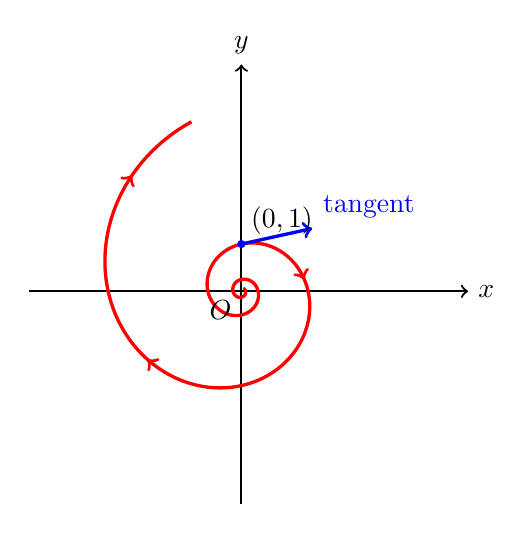
\begin{tikzpicture}[scale=0.6]
    % Axes
    \draw[->,thick] (-4.5,0) -- (4.8,0)
        node[right] {$x$};
    \draw[->,thick] (0,-4.5) -- (0,4.8)
        node[above] {$y$};

    % Schematic: slower radial growth makes the turns visible.
    % All arrows indicate increasing time.
    \draw[
        red,very thick,
        postaction={decorate},
        decoration={
            markings,
            mark=at position 0.35 with {\arrow{>}},
            mark=at position 0.65 with {\arrow{>}},
            mark=at position 0.9 with {\arrow{>}}
        }
    ]
        plot[domain=-12:6,samples=600,variable=\t]
        ({exp(0.22*\t)*sin(deg(\t))},
         {exp(0.22*\t)*cos(deg(\t))});
    % Tangent to the plotted schematic at (0,1)
    \draw[->,blue,very thick]
        (0,1) -- (1.5,1.33)
        node[above right] {tangent};

    \fill[blue] (0,1) circle (2.5pt);
    \node[above right] at (0,1) {$(0,1)$};
    \node[below left] at (0,0) {$O$};
\end{tikzpicture}

\end{center}
\end{example}


\end{document}